\documentclass[a4paper,chapter,atbegshi]{oblivoir}
\usepackage[dbl4x6]{fapapersize}
\usepackage{amsmath,amssymb,amsfonts,amsthm}
\usepackage{graphicx,xcolor,caption}
\usepackage{braket,hyperref,nicematrix}
\usepackage{euler,enumitem,tikz}
\usepackage{quantikz,wrapfig,mdframed}
\usetikzlibrary{arrows.meta}
\setlist{nosep}
\hypersetup{
  colorlinks=true,linkcolor=teal,filecolor=magenta,urlcolor=cyan,
}
\title{\texttt{Introduction to Quantum Information Science} 학습일지}
\author{김태원}
\date{최초 작성 : 2023년 8월 29일 \\ 최근 편집 : \today}

\begin{document}
\maketitle
\break
\tableofcontents
\chapter{유니타리 변환}
파인만{\tiny Richard Feynman}이 말하길 이중슬릿{\tiny double slit} 실험으로
양자역학을 전부 요약할 수 있다.

두 개의 슬릿{\tiny slit}을 지닌 벽에 광자{\tiny photons}를 하나씩 쏜다고 하자.
두 슬릿 모두 열릴 때 광자가 특정 구간에 부딪히는 확률을 $P$, 1번 슬릿만
열릴 때 광자가 특정 구간에 부딪히는 확률을 $P_1$, 2번 슬릿만 열릴 때 광자가
특정 구간에 부딪히는 확률을 $P_2$라고 하자. 확률론에 따르면 당연히 $P=P_1+P_2$다.
그런데 실험 결과에 따르면 $P\neq P_1+P_2$다. 다시 말해 자연스러운 확률론은 자연의 
현상을 설명하지 못한다.

고전적인 확률론이 자연을 충분하게 설명하지 못하는데도 자연스러워 보이는 이유는 
\textbf{결어긋남\tiny decoherence}이라는 현상에서 비롯한다. 이를테면 상자를
열었을 때 슈뢰딩거의 고양이는 생과 사의 \emph{중첩\tiny superposition}으로
나타나지 않는다. 고양이가 제 환경과 끊임없이 상호작용하기 때문이다. 고양이와
환경 간의 상호작용은 고양이 계{\tiny system}의 정보를 누설하는 반면 양자
중첩은 입자나 입자들의 군이 환경과 \emph{고립\tiny isolated}될 때 일어난다.

똑똑한 물리학자들이 이중슬릿 같은 실험을 통해 관찰한 바, 자연은 고전적인 확률
$P\in[0,1]$가 아니라 어떤 파동함수를 따른다. 그리고 이런 파동함수를 포착하는 
개념이 바로 \textbf{진폭\tiny amplitude} $\alpha\in\mathbb{C}$다. 양자역학에서
확률은 진폭을 사용해 \textbf{보른 규칙\tiny Born Rule}으로 정의된다. 보른 규칙은
양자계의 파동함수를 아우르는 슈뢰딩거 방정식의 해를 해석할 수 있는 유일한
방법으로 1926년 보른{\tiny Max Born}이 제시한 공리다.
\begin{equation}\label{eq:11}
  P = |\alpha|^2 = \textrm{Real}(\alpha)^2+\textrm{Imaginary}(\alpha)^2
\end{equation}
진폭으로 이중슬릿 실험을 다시 확인하겠다. 두 슬릿 모두 열릴 때 광자가
특정 구간에 부딪히는 진폭을 $\alpha$, 1번 슬릿만 열릴 때 광자가 특정 구간에
부딪히는 진폭을 $\alpha_1$, 2번 슬릿만 열릴 때 광자가 특정 구간에
부딪히는 진폭을 $\alpha_2$라고 하자. 이때 등식 $\alpha=\alpha_1+\alpha_2$는 모순을
유도하지 않는다. $\alpha_1=a_1+b_1i, \alpha_2=a_2+b_2i$에 대해
\begin{align*}
  \alpha &= \alpha_1 + \alpha_2 \\
  \Rightarrow  P &= |\alpha|^2 \quad\quad\quad\quad[\textrm{보른 규칙}]\\ 
      &= |\alpha_1+\alpha_2|^2\\
      &= \textrm{Re}(\alpha_1+\alpha_2)^2+\textrm{Im}(\alpha_1+\alpha_2)^2\\
      &= (a_1+a_2)^2+(b_1+b_2)^2 \\
      &= (a_1^2+2a_1a_2+a_2^2)+(b_1^2+2b_1b_2+b_2^2) \\
      &= (a_1^2+b_1^2)+(a_2^2+b_2^2)+2(a_1a_2+b_1b_2)\\
      &= \textrm{Re}(\alpha_1)^2+\textrm{Im}(\alpha_1)^2+
      \textrm{Re}(\alpha_2)^2+\textrm{Im}(\alpha_2)^2+\overline{\alpha_1}\alpha_2+
      \alpha_1\overline{\alpha_2}\\
      &=|\alpha_1|^2+|\alpha_2|^2+\overline{\alpha_1}\alpha_2+
          \alpha_1\overline{\alpha_2} 
\end{align*}
복소수 진폭 $\alpha$가 음수일 수 있으므로 아래 상황이 가능하기 때문이다.
\[
  \alpha_1 := \frac{1}{2}, \alpha_2 := -\frac{1}{2} \Rightarrow
  \begin{cases}
    |\alpha_1|^2 = \frac{1}{4}, |\alpha_2|^2=\frac{1}{4} \\
              |\alpha=\alpha_1+\alpha_2|^2=0
  \end{cases}
\]
이처럼 두 상태의 진폭은 서로 소거할 수 있다. \textbf{간섭\tiny
interference}이라는 현상이다. 간섭은 간단한 선형대수학으로 설명된다.
우선 2-노름{\tiny norm} $\alpha^2+\beta^2=1$을 충족하는 벡터 $(\alpha,\beta)$가
원을 형성한다는 사실에 주목한다. 
\begin{figure}[h]
\begin{center}
  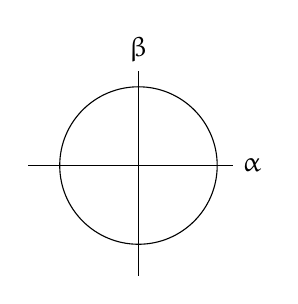
\begin{tikzpicture}
    \draw[fill=none](0,0)circle(1.0); 
    \draw[](0,-1.4)--(0,1.2) node[above]{$\beta$};
    \draw[](-1.4,0)--(1.2,0) node[right]{$\alpha$};
  \end{tikzpicture}
  \caption{유클리드 노름\label{fig:1-1}}
\end{center}
\end{figure}
2-노름을 유클리드 노름{\tiny Euclidean norm}이라고 부르기도 한다.
원은 임의의 $\alpha,\beta$에 대해 형성되기에 어느 유클리드 노름 단위
벡터를 다른 유클리드 노름 단위 벡터로 사상하는{\tiny maps to} 행렬 혹은 변환이
존재한다. 바로 \textbf{유니타리 행렬\tiny unitary matrix}이다.
또한 여기서 `유클리드 노름 단위 벡터'가 바로 \textbf{큐비트\tiny qubit}다. 

물리학자들은 디락{\tiny Paul Dirac}이 도입한 브라-켓{\tiny bra-ket} 표기법으로
큐비트를 나타낸다. 켓{\tiny ket} $\ket{\psi}$과 브라{\tiny bra} $\bra{\psi}$는
아래와 같다.
 \[
   \ket{\psi} = \alpha\ket0+\beta\ket1 = \begin{pmatrix}\alpha\\\beta\end{pmatrix}
  =\alpha\begin{pmatrix}1\\0\end{pmatrix}+\beta\begin{pmatrix}0\\1\end{pmatrix},
  \quad
  \bra{\psi} = \overline{\alpha}\bra0 +\overline{\beta}\bra1=
   \begin{pmatrix}\overline{\alpha}&\overline{\beta}\end{pmatrix}
 \]
이에 유클리드 노름 $\|\psi\|^2$가 자연스럽게 정의될 수 있다. 
 \[
   \|\psi\|^2 = \begin{pmatrix}\overline{\alpha}&\overline{\beta}\end{pmatrix}
   \begin{pmatrix}\alpha\\\beta\end{pmatrix}=|\alpha|^2+|\beta|^2
 \]
 내적 $\braket{\psi|\phi}$는 아래 성질을 만족한다.
 \begin{align*}
   \braket{\psi|\phi} &= 
   \begin{pmatrix}\overline{\alpha_1} &\overline{\beta_1}\end{pmatrix}
   \begin{pmatrix}\alpha_2\\\beta_2\end{pmatrix} \\
    &= \overline{\alpha_1}\alpha_2+\overline{\beta_1}\beta_2\\
    &=\overline{\alpha_1}\overline{\overline{\alpha_2}}+
    \overline{\beta_1}\overline{\overline{\beta_2}} \\
    &= \begin{pmatrix}\overline{\overline{\alpha_2}} & \overline{\overline{\beta_2}}\end{pmatrix}
   \begin{pmatrix}\overline{\alpha_1}\\\overline{\beta_2}\end{pmatrix}
   = \overline{\braket{\phi|\psi}}
 \end{align*}
 여기서 $\alpha$는 $\ket{0}$이라는 결과에 대한 진폭이고 $\beta$는 $\ket{1}$이라는
결과에 대한 진폭이다. 따라서 상태 $\ket\psi$에서 상태 $\ket\phi$에 이르는
확률 $P(\ket\phi)$에 대해 보른 규칙을 다시 서술할 수 있다.
\[
  P(\ket\phi)=|\braket{\psi|phi}|^2
\]
이에 행렬을 $45^{\circ}$ 즉 $\frac{\pi}{4}$만큼 회전하며 노름을 보존하는
아래 같은 유니타리 행렬이 있다고 하자.
\[
  \begin{pmatrix}
    \cos\frac{\pi}{4} &-\sin\frac{\pi}{4}\\
    \sin\frac{\pi}{4} &\cos\frac{\pi}{4}
  \end{pmatrix}
  = \begin{pmatrix}
    \frac{1}{\sqrt{2}} &-\frac{1}{\sqrt{2}} \\
    \frac{1}{\sqrt{2}} &\frac{1}{\sqrt2}
  \end{pmatrix}
\]
$\ket0$를 위 유니타리 행렬로 변환한다.
\begin{equation}\label{eq:1-2}
  \begin{pmatrix}
    \frac{1}{\sqrt{2}} &-\frac{1}{\sqrt{2}} \\
    \frac{1}{\sqrt{2}} &\frac{1}{\sqrt2}
  \end{pmatrix}
  \begin{pmatrix}
    1\\0
  \end{pmatrix}
  =\begin{pmatrix}
    \frac{1}{\sqrt2}\\\frac{1}{\sqrt2}
  \end{pmatrix}
\end{equation}
$\frac{1}{\sqrt2}\ket{0}+\frac{1}{\sqrt2}\ket{1}$을 다시 위 유니타리 행렬로
변환한다.
\[
  \begin{pmatrix}
    \frac{1}{\sqrt{2}} &-\frac{1}{\sqrt{2}} \\
    \frac{1}{\sqrt{2}} &\frac{1}{\sqrt2}
  \end{pmatrix}
  \begin{pmatrix}
    \frac{1}{\sqrt2}\\\frac{1}{\sqrt2}
  \end{pmatrix}
  =\begin{pmatrix}0\\1\end{pmatrix}=\ket{1}
\]
즉 무작위 상태 $\frac{1}{\sqrt2}\ket{0}+\frac{1}{\sqrt2}\ket{1}$에 위 유니타리
행렬과 같은 무작위 연산을 적용하면 $\ket{1}$이라는 결과가 결정론적{\tiny
deterministic}으로 나온다. 여기 무작위 연산을 다시 적용하여 나타난 무작위 상태
 $-\frac{1}{\sqrt2}\ket{0}+\frac{1}{\sqrt2}\ket{1}$에 무작위 연산을 또다시
 적용하면 $\ket{0}$이라는 결과가 결정론적으로 나온다. 이것이 앞서 언급한
 \textbf{간섭} 개념의 선형대수학적 바탕이다. 

 여기서 $\ket{0}$이라는 결과를 결정론적으로 도출하는 유니타리 행렬이 
 $\frac{1}{\sqrt2}\ket0-\frac{1}{\sqrt2}\ket{1}$이라는 사실에 주목한다.
 이 사실을 \textbf{경로\tiny
 path}가 두 개 존재하여 한 경로는 음의 진폭 $-\frac{1}{\sqrt2}$를 지니고 
 다른 경로는 양의 진폭 $\frac{1}{\sqrt2}$을 지녀 두 경로는 \textbf{파괴적
 간섭\tiny destructive interference} 관계에 놓인다고 표현한다. 
 반면 $\ket{1}$이라는 결과를 결정론적으로 도출하는 경로는 모두 양의 진폭
 $\frac{1}{\sqrt2}$을 지녀 \textbf{구성적 간섭\tiny constructive interference}
 관계다.

 이제 그림 \ref{fig:1-1}상의 원을 다시 그린다.
\begin{figure}[h]
\begin{center}
  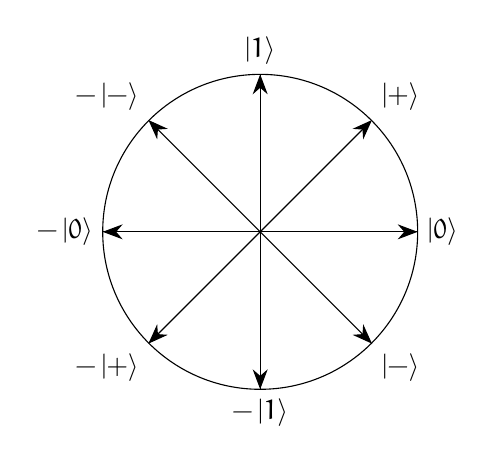
\begin{tikzpicture}
    \draw[fill=none](0,0)circle(2.0);
    \draw[-{Stealth[scale=1.5]}] (0,0)--(0,2);
    \draw[-{Stealth[scale=1.5]}] (0,0)--(-2,0) node[left]{$-\ket0$};
    \draw[-{Stealth[scale=1.5]}] (0,0)--(1.42,1.42) node[above right]{$\ket+$};
    \draw[-{Stealth[scale=1.5]}] (0,0)--(2,0);
    \draw[-{Stealth[scale=1.5]}] (0,0)--(-1.42,1.42) node[above left]{$-\ket-$};
    \draw[-{Stealth[scale=1.5]}] (0,0)--(1.42,-1.42) node[below right]{$\ket-$};
    \draw[-{Stealth[scale=1.5]}] (0,0)--(0,-2) node[below]{$-\ket1$};
    \draw[-{Stealth[scale=1.5]}] (0,0)--(-1.42,-1.42) node[below left]{$-\ket+$};
    \draw[](0,-2.0)--(0,2.0) node[above]{$\ket1$};
    \draw[](-2.0,0)--(2.0,0) node[right]{$\ket0$};
  \end{tikzpicture}
  \caption{직교 행렬\label{fig:1-2}}
\end{center}
\end{figure}
여기서 $\{\ket+,\ket-\}$는 \emph{아다마르 기저\tiny Hadamard basis}라고 하며
$45^{\circ}$ 회전 유니타리 변환 과정 \ref{eq:1-2}에서 이미 봤다. 
\[
  \begin{pmatrix}\frac{1}{\sqrt2}\\\frac{1}{\sqrt2}\end{pmatrix}=\ket+ =
  \frac{\ket0+\ket1}{\sqrt2},\quad\begin{pmatrix}\frac{1}{\sqrt2}\\
  -\frac{1}{\sqrt2}\end{pmatrix} = \ket-=\frac{\ket0-\ket1}{\sqrt2}
\]
아다마르 기저는 \textbf{아다마르 게이트}{\tiny gate}\footnote{유니타리 변환을
게이트라고 부르기도 한다.} $H:\{\ket0,\ket1\} \rightarrow
\{\ket+,\ket-\}$ 를 형성한다. 이를테면 $\ket0$에 $H$를 적용한 결과는 아래와 같다.
\[
  H\ket0=\frac{1}{\sqrt2}\begin{pmatrix}1&1\\1&-1\end{pmatrix}
  \begin{pmatrix}1\\0\end{pmatrix} =
  \begin{pmatrix}\frac{1}{\sqrt2}\\\frac{1}{\sqrt2}\end{pmatrix}=\ket+
\]
그림 \ref{fig:1-2}에서 확인할 수 있는 사실은 $\frac{\pi}{4}$
회전과 반사만으로 여덟 가지 상태를 나타낼 수 있다는 것과 원의 방정식에 의해
유니타리 변환이 유클리드 노름을 보존한다는 것이다. 가령 임의의 유니타리 행렬
$U$의 복소전치행렬 $U^{\dagger}$를 $U$로 변환하면 항등행렬 $I$가 나온다.
\[
  \braket{\psi|\psi} = (\ket{\psi})^{\dagger}\ket{\psi} 
              = (U\ket{\psi})^{\dagger}U\ket{\psi}
              =\braket{\psi|U^{\dagger}U|\psi} 
  \iff\forall\ket{\psi},U^{\dagger}U= I
\]
유니타리 변환은 선형변환이기도 해서 $U(c\ket0)=cU\ket0$이 임의의 상수 $c$에 
대해 성립할 수 있다. 여기서 $c$가 어떤 $\theta$에 대해 오일러 공식 
$e^{i\theta}=\cos\theta+i\sin\theta$\footnote{오일러 공식은 슈뢰딩거
방정식을 비롯해 양자역학에서 중요한 파동-삼각함수를 지수함수로 변환할 수 있도록
하며, 복소평면에서 일정한 속도로 원운동하는 물체의 위치 방정식으로 정의된다.}를
만족하면 \textbf{전역위상\tiny global phase}이라고 한다. 다만 $\ket{\psi}$와 
$e^{i\theta}\ket{\psi}$가 물리적으로 구분될 수 없기에 전역위상은
관찰불가능하다. 전역위상이 관찰가능하다는 말은 큐비트와 같은
양자계에 어떤 스칼라를 곱해서 우주 전체를 살짝 옮길 수 있다는
소리와 같다. 이에 반해 관찰 가능한 것은 바로 \textbf{상대위상\tiny relative
phase}이다. 가령 $\ket+$와 $\ket-$라는 두 상태 간에는 상대위상차이가 관측될 수
있는데, $\ket-$에서 $\ket+$에 이르는 일련의 유니타리 연산들이 존재하기 때문이다.

관찰 혹은 측정{\tiny measurment}과 유니타리 연산 간에 차이가 존재하는
셈이다. 유니타리 변환이 (그 복소전치행렬로 인해) 가역{\tiny invertible}이고
결정론적이며 (복소수 행렬이기에 모든 $a$에 대해 $\sqrt{a}$를 내놓을 수 있어서)
연속적인 반면, 측정은 비가역{\tiny irreversible}이고 확률론적, 비연속적이다.
이처럼 판이한 유니타리 변환과 측정을 이어주는 것이 바로 유클리드 노름이다.
유니타리 변환은 유클리드 노름을 보존하고 측정은
유클리드 노름으로 결정되는 확률을 제공한다. 그리고 이에 따른 연속과 비연속,
결정론과 확률론의 상호작용을 소진하는 사고실험이 바로 \emph{튜링의
역설} 혹은 \textbf{양자 제논 효과}다.

$\ket0$이나 $\ket1$로 설정된 큐비트가 있다고 하겠다. 이 큐비트에 유니타리
변환을 전혀 사용하지 않으면서 상태를 바꿀 수 있을까? 아주 작은 $\epsilon$에 
대해 $\{\ket0,\ket1\}$에서 $\epsilon$만큼 회전한 기저는 아래처럼 측정할 수 있다.
\begin{align*}
  \begin{aligned}
  \ket0\mapsto\ket{v}&= \cos\epsilon\ket0+\sin\epsilon\ket1\\
  \Rightarrow 
    P(\ket{v})&=|\braket{0|v}|^2 \\
              &=\left|\begin{pmatrix}1,0\end{pmatrix}
              \begin{pmatrix}\cos\epsilon\\\sin\epsilon\end{pmatrix}\right|^2 \\
              &=|\cos\epsilon|^2 \approx{\biggl(1-\frac{\epsilon^2}{2}\biggr)^2}\\
              &= 1-\epsilon^2+\frac{\epsilon^4}{4}
              \approx 1-\epsilon^2 \\
  \end{aligned}
  \begin{aligned}
  \ket1\mapsto\ket{w}&=-\sin\epsilon\ket0+\cos\epsilon\ket1\\
    P(\ket w)&=|\braket{1|w}|^2 \\
              &=\left|\begin{pmatrix}0,1\end{pmatrix}
              \begin{pmatrix}-\sin\epsilon\\\cos\epsilon\end{pmatrix}\right|^2\\
              &=|\cos\epsilon|^2 \approx \biggl(1-\frac{\epsilon^2}{2}\biggr)^2\\
              &= 1-\epsilon^2+\frac{\epsilon^4}{4}
              \approx1-\epsilon^2
  \end{aligned}
\end{align*}
큐비트가 $\epsilon$만큼 회전할 수 있는 확률은 $\epsilon$이 감소할수록 
증가\footnote{근사값의 유도에 관해서는 \href{https://en.wikipedia.org/wiki/Small-angle_approximation}{작은 각도 근사}를 참고하라.}한다.
그러니 이 절차를 대략 $\frac{1}{\epsilon}$번 반복하며 매번 $\epsilon$만큼 
회전하면, $\ket0$을 아주 천천히 $\ket1$로 옮길 수 있다. 이 과정이
성공하지 \emph{않을} 확률은 $1-(1-\epsilon^2)=\epsilon^2$에 $\frac{1}{\epsilon}$을
곱한 $\epsilon$이다. 그리고 $\epsilon$은 가정에 의해 극미량이다.
따라서 유니타리 변환이 없더라도 아주 높은 확률로 상태를 바꿀 수 있다. 

그런데 이게 무슨 소리인가? 비유하자면, 홍길동의
$\ket{\textrm{미혼}}$ 상태를 $\ket{\textrm{기혼}}$ 상태로 바꾸는
유니타리 변환 수준의 깔끔한 방법은 당장 김철수와 서류상
혼인신고하는 것이다. 이 방법은 지금 어렵다고 할 때,
홍길동이 김철수를 1년간 그냥 지켜보다가 어느 날 갑자기 프로포즈하는
쪽보다는 홍길동이 1년을 $\frac{1}{\epsilon}$ 정도로 아주 잘게 나눠 $\epsilon$
만큼의 애정 표현을 반복하는 쪽의 결혼 확률이 더 높을 것이다.

다음 예는 \textbf{엘리추르-바이드만 폭탄\tiny Elitzur-Vaidman Bomb}으로,
양자 공항이 배경이다. 화물에 폭탄이 존재하는 것 같은데, 폭탄이 있다면
화물을 여는 순간 폭발할 것이 분명하다. 폭탄이 폭발할 확률을 최소화할 수 있을까?

우선 $\ket0$을 초기 상태로 둔다. 화물 확인이라는 행동은 회전 
$R_{\epsilon}$으로 정의한다. 
\[
  R_{\epsilon} = \begin{pmatrix}\cos\epsilon&-\sin\epsilon\\
  \sin\epsilon &\cos\epsilon\end{pmatrix}
\]
폭탄이 없다면, 그대로 $\cos\epsilon\ket0+\sin\epsilon\ket1$이다. 폭탄이 있다면,
폭탄은 $\{\ket0,\ket1\}$을 기저로 측정된다. 다시 말해 회전-확인의 결과가
$\ket0$이라면 폭탄이 폭발하지 않은 것이다. 그리고 결과가 $\ket1$이라면
폭탄이 폭발한 것이다. 

초기 상태 $\ket0$에 대해 화물을 한 번 확인-$R_{\epsilon}$한 결과는
$\cos\epsilon\ket0+\sin\epsilon\ket1$이다. 폭탄이 존재할 때,
 폭탄이 폭발할 확률 $P(1)$은 $\cos\theta\ket0+\sin\epsilon\ket1$이
$\ket1$로 관측될 확률과 같다. 
\begin{align*}
  P(1) &= |\braket{b|1}|^2 \\
       &= \left|\begin{pmatrix}\cos\epsilon &\sin\epsilon\end{pmatrix}
       \begin{pmatrix}0\\1\end{pmatrix}\right|^2\\
       &=|\sin\epsilon|^2 \approx \epsilon^2
\end{align*}
따라서 이 과정을 대략 $\frac{\pi}{2\epsilon}$번\footnote{여기서 
$\frac{\pi}{2\epsilon}$은 $90^{\circ}$보다 아주 약간 작은 각도로, 그림 
\ref{fig:1-2}의 원에서 `$\ket1$' 직전에 해당한다.} 
반복하며 매번 $R_{\epsilon}$을 적용하면, 존재하는 폭탄이 터지는 확률은
$\frac{\pi}{2\epsilon}\epsilon^2 =\frac{\pi}{2}\epsilon$에 불과하다. 따라서
양자 공항에서는 대단히 높은 확률로 폭탄이 폭발하지 않는다.

\section*{양자회로}
그림 \ref{fig:1-3}은 $\ket1$로 초기 상태를 설정한 다음 두 아다마르 게이트를
적용하여 표준기저 $\{\ket0,\cdots,\ket{N-1}\}$상의 측정으로 종결하는 
양자회로다. 양자회로는 여러 큐비트에 대한 연산을 표기할 수도 있다. 
그림 \ref{fig:1-4}는 이중 큐비트 게이트 $U$에 대해 첫 번째 큐비트로 
아다마르 게이트를 적용한 다음 두 큐비트를 모두 측정하는 양자회로다.
\begin{figure}[h]
\begin{minipage}{0.48\textwidth}
\centering
\begin{quantikz}
  \lstick{$\ket1$}&\gate{H}&\gate{H}&\meter{} 
\end{quantikz}
\caption{양자 회로 예제\label{fig:1-3}}
\end{minipage}\hfill
\begin{minipage}{0.48\textwidth}
\centering
  \begin{quantikz}
    \lstick{$\ket0$}&\gate[2]{U}&\gate{H}&\meter{} \\
    \lstick{$\ket0$}& &\qw &\meter{} 
  \end{quantikz}
  \caption{이중 양자 회로 예제\label{fig:1-4}}
\end{minipage}
\end{figure}

\noindent
그림 \ref{fig:1-5} 좌측의 양자회로는 제어{\tiny controlled} 게이트를 사용한다. 
첫 줄에 놓인 $\bullet-\oplus$는 제어 NOT 혹은 CNOT 게이트를 나타내고 이는
첫 비트 혹은 제어 큐비트가 $\ket1$이면 두 번째 큐비트를 반전{\tiny flip}한다. 그 다음 줄에 놓인 $\bullet- U$는 임의의 $U$에 대해 제어 $U$ 게이트를 
나타내며 제어 큐비트가 $\ket1$이면 $U$를 적용한다.
\begin{figure}[h]\centering
  \begin{quantikz}
    & \ctrl{1} & \ctrl{1} & \targ{} & \qw \\
    & \targ{} & \gate{U} & \ctrl{-1} & \qw
  \end{quantikz}
  여기서
  \begin{quantikz}
    &\targ{}&\qw \\
    &\ctrl{-1}&\qw
  \end{quantikz}
  =\begin{quantikz}
    &\gate{H}&\ctrl{1}&\gate{h}&\qw\\
    &\gate{H}&\targ{}&\gate{h}&\qw
  \end{quantikz}
  \caption{제어 양자 회로 예제\label{fig:1-5}}
\end{figure}
마지막 줄은 우측 도면과 같다.
\chapter{부분 측정 규칙}
두 개의 큐비트로 구성한 $\ket{\psi} = \alpha\ket{00}+\beta\ket{01}+
\gamma\ket{10}+\delta\ket{11}$가 있다. 이때
첫 큐비트는 $\ket0$이라는 정보가 주어지면 두 번째
큐비트는 $\ket0$과 $\ket1$ 가운데 하나일 수밖에 없다.
다시 말해 $\ket{00}$이나 $\ket{01}$만이 가능하며
두 번째 큐비트를 아래 중첩으로 나타낼 수 있다. 
\begin{equation}\label{eq:2-1}
  \ket0\otimes\frac{\alpha\ket0+\beta\ket1}{\sqrt{|\alpha|^2+|\beta|^2}}
  = \begin{bmatrix}1\\0\end{bmatrix}\otimes
  \begin{bmatrix}\alpha\\\beta\end{bmatrix}\frac{1}{\sqrt{|\alpha|^2+|\beta|^2}}
  = \begin{bmatrix}\alpha\\\beta\\0\\0\end{bmatrix}\frac{1}{\sqrt{|\alpha|^2+|\beta|^2}}
\end{equation}
여기서 $\sqrt{|\alpha|^2+|\beta|^2}$로 나누는 과정을 
정규화{\tiny normalization}라고
부른다. $\ket{\psi}$는 $\alpha,\beta$가 아니라 $\alpha,\beta,\gamma,\delta$에
대해 노름의 조건 $\sqrt{|\alpha|^2+|\beta|^2+|\gamma|^2+|\delta|^2}=1$을 지키도록
정의되었다. 따라서 $\alpha$와 $\beta$만 있어도 아래처럼 노름의 조건이 
지켜져야 한다. 
\[
  \Bigg\lvert\frac{\alpha}{\sqrt{|\alpha|^2+|\beta|^2}}\Bigg\rvert^2 +
  \Bigg\lvert\frac{\beta}{\sqrt{|\alpha|^2+|\beta|^2}}\Bigg\rvert^2
  =
  \frac{|\alpha|^2+|\beta|^2}{|\alpha|^2+|\beta|^2}=1
\]
아무튼 이처럼 한 양자정보가 주어지면 나머지 양자정보만
따로 떼어내서 측정할 수 있다는 규칙을 
\textbf{부분측정규칙\tiny partial measurement rule}이라고 부른다.
가령 ``두 번째 큐비트에 NOT 게이트를 적용하라''는
말을 아래처럼 나타낼 수 있고
\[
  I\otimes \textrm{NOT} = \begin{bmatrix}1 & 0 \\ 0 & 1\end{bmatrix}
  \otimes \begin{bmatrix}0 & 1 \\ 1 & 0\end{bmatrix}=
  \begin{bmatrix}0&1&0&0\\1&0&0&0\\0&0&0&1\\0&0&1&0\end{bmatrix}
\]
``모든 큐비트에 아다마르 게이트를 적용하라''는 말은 아래처럼 나타낼 수 있다.

\[
  H\otimes H=
  \frac{1}{\sqrt2}\begin{bmatrix}1&1\\1&-1\end{bmatrix}\otimes
  \frac{1}{\sqrt{2}}\begin{bmatrix}1&1\\1&-1\end{bmatrix}=\frac{1}{2}
  \begin{bNiceMatrix}[first-col, first-row]
    & \scriptstyle00 & \scriptstyle01 & \scriptstyle10 & \scriptstyle11 \\
    \scriptstyle00 & 1 & 1 & 1 & 1 \\
    \scriptstyle01 & 1 & -1 & 1 & -1 \\
    \scriptstyle10 & 1 & 1 & -1 & -1 \\
    \scriptstyle11 & 1 & -1 & -1 & 1
  \end{bNiceMatrix}
\]
여기서 $00$이라는 첨자를 지니는 행을 $H\otimes H\ket{00}=
\ket{++}$이라는 텐서곱으로 생각할 수 있다. 마찬가지로 $01$이라는 첨자를 지니는
두 번째 행을 $H\otimes H\ket{01}=\ket{+-}$이라는 텐서곱으로
받아들일 수 있다.
\[
  \ket{+-}=\ket{+}\otimes\ket{-}=
  \frac{\ket0+\ket1}{\sqrt{2}}\otimes\frac{\ket0-\ket1}{\sqrt2}=
  \begin{bmatrix}\frac{1}{\sqrt{2}}\\\frac{1}{\sqrt2}\end{bmatrix}\otimes
  \begin{bmatrix}\frac{1}{\sqrt2}\\-\frac{1}{\sqrt2}\end{bmatrix} =
  \begin{bmatrix}\frac{1}{2}\\-\frac{1}{2}\\\frac{1}{2}\\-\frac{1}{2}\end{bmatrix}
  = \frac{1}{2}\begin{bNiceMatrix}[first-row] 
  \scriptstyle01\\1\\-1\\1\\-1\end{bNiceMatrix}
\]
이처럼 2-큐비트 유니타리를 1-큐비트 유니타리의 텐서곱으로 구성할 수 있다.
다만 CNOT 게이트는 예외다. CNOT은 첫 번째 큐비트가 $0$이면 두 번째
큐비트를 놔두고 첫 번째 큐비트가 $1$이면 두 번째 큐비트를 반전하는 게이트다.
\[
  CNOT = \begin{bNiceMatrix}[first-col, first-row]
    & \scriptstyle00 & \scriptstyle01 & \scriptstyle10 & \scriptstyle11 \\
    \scriptstyle00 & 1 & 0 & 0 & 0 \\
    \scriptstyle01 & 0 & 1 & 0 & 0 \\
    \scriptstyle10 & 0 & 0 & 0 & 1 \\
    \scriptstyle11 & 0 & 0 & 1 & 0
  \end{bNiceMatrix}
\]
즉 CNOT은 한 큐비트가 다른 큐비트한테 영향을 미친다. CNOT의
이런 성질을 사용하는 특이한 상태가 있다. 바로 \textbf{벨 쌍\tiny
Bell Pair} 혹은 \textbf{EPR 쌍} 혹은 \textbf{싱글렛\tiny singlet}이다.
\[
  (CNOT)(H\otimes I)
  \begin{bmatrix}1\\0\\0\\0\end{bmatrix}
    =CNOT \frac{1}{\sqrt{2}}
    \begin{bmatrix}1&0&1&0\\0&1&0&1\\1&0&-1&0\\0&1&0&-1\end{bmatrix}
    \begin{bmatrix}1\\0\\0\\0\end{bmatrix}
  \longrightarrow 
  CNOT\begin{bmatrix}\frac{1}{\sqrt2}\\0\\\frac{1}{\sqrt2}\\0\end{bmatrix}
  \longrightarrow
  \begin{bmatrix}\frac{1}{\sqrt{2}}\\0\\0\\\frac{1}{\sqrt2}\end{bmatrix}
\]
CNOT의 첫 큐비트와 두 번째 큐비트를 텐서곱으로 분해할 수 없으므로 벨 쌍
또한 첫 큐비트와 두 번째 큐비트를 텐서곱으로 분해할 수 없다. 이런 
상태를 \textbf{얽힘\tiny entanglement} 혹은 \emph{순수 상태}라고 부른다. EPR 쌍은
이름만 무려 세 개인 만큼 중요한 상태이기 때문에 회로와 브라켓도 기억해 둔다.

\begin{figure}[h]
  \centering
  \begin{minipage}{0.3\textwidth}
  \begin{quantikz}
  \lstick{$\ket0$}&\gate{H}&\ctrl{1}&\qw\\
  \lstick{$\ket0$}&\qw&\targ{}&\qw
  \end{quantikz}
\end{minipage}
\begin{minipage}{0.5\textwidth}
\[
  \ket{00}\longrightarrow\ket+\otimes\ket0=\frac{\ket{00}+\ket{10}}{\sqrt2}
  \longrightarrow\frac{\ket{00}+\ket{11}}{\sqrt2}
\]
\end{minipage}
\caption{EPR 쌍}
\end{figure}
\noindent
얽힘은 지금껏 설명한 기초개념들의 필연적인 귀결이다. 또한 얽힘은 (EPR 쌍에서
`E'를 맡은) 아인슈타인이 양자역학에 신경질을 부린 이유다. 여타 물리학자와
다르게 아인슈타인, 포돌스키{\tiny Boris Podolsky}, 로젠{\tiny Nathan Rosen}의
신경을 긁은 이야기는 아래와 같다.

\begin{mdframed}
달에 앨리스가 있고 지구에 밥이 있다고 하자. 앨리스와 밥은 각각 큐비트를
하나씩 지닌다. 그리하여 두 큐비트에 EPR 쌍 $\frac{\ket{00}+\ket{11}}{\sqrt2}$으로
얽힘을 부여한다. 그렇다면 앨리스가 자신의 큐비트의 상태를 측정한
\textbf{바로 그때} 앨리스는 밥이 관측할 큐비트의 상태가 $\ket{+}$이거나
$\ket{-}$이라는 사실을 알 수 있다. 얽힘 탓이다.
\end{mdframed}

1935년 EPR 삼인방은 이를 \snm{물리적 실재에 대한 양자역학적 기술이
완전하다고 여길 수 있는가?}{\tiny Can Quantum-Mechanical Description of
Physical Reality be Considered Complete?}라는 논문으로 발표한다. 요,
달에서 앨리스가 자신의 큐비트를 측정한 바로 그 순간 지구에서 밥이
측정할 큐비트의 상태에 관한 지식을 취할 수 있다. 일종의 통신{\tiny 
communication}이다. 다만 즉각적인 통신이다. 그래서 빛보다 빠르다. 
하지만 상대성이론에 따르면 빛보다 빠른 것은 없다. 따라서 얽힘이라는
개념에는 문제가 있다.

EPR 삼인방은 논증을 강화하기 위해 앨리스가 얽힘을 측정하는 기저를 바꾼
즉시 밥의 큐비트도 그 기저에 따라 붕괴한다는 예를 든다. 앨리스가 EPR 쌍에
아다마르 게이트를 적용해서 $\{\ket0,\ket1\}$을 기저로 측정한다고 하자.
\begin{align*}
  &(H\otimes I)\left(\frac{\ket{00}+\ket{11}}{\sqrt2}\right)
  =\frac{1}{\sqrt2}
  \begin{bmatrix}
    1&0&1&0 \\ 0&1&0&1 \\ 1&0&-1&0 \\0&1&0&-1
  \end{bmatrix}
  \frac{1}{\sqrt2}\begin{bmatrix}1\\0\\0\\1\end{bmatrix}
  =
  \frac{1}{2}\begin{bmatrix}1\\1\\1\\-1\end{bmatrix}\\=&\;
  \frac{\ket{00}+\ket{01}+\ket{10}-\ket{11}}{2} 
\end{align*}
부분측정규칙 \ref{eq:2-1}에 의해 앨리스가 $\ket0$을 보면 밥의 큐비트는
$\ket0$이나 $\ket1$로 붕괴하고 앨리스가 $\ket1$을 보면 밥의 큐비트는 
$\ket0$이나 $\ket1$로 붕괴한다. 반면 앨리스가 EPR 쌍을 $\{\ket+,\ket-\}$로
측정했을 때 $\ket+$를 보면 밥의 큐비트는 $\ket+$나 $\ket-$로 붕괴하고
앨리스가 $\ket-$를 보면 밥의 큐비트는 $\ket+$나 $\ket-$로 붕괴한다.

얽힘이 상대성이론을 뿌리부터 전면 부인하다는 소리다.
하지만 얽힘 혹은 순수상태가 양자역학적 상태의 전부는 아니다. 순수상태는
\textbf{혼합상태\tiny mixed states}의 일종일 따름이다. 혼합상태란
양자 상태 $\ket{\psi}$에 대한 확률 $p_i$의 분포 $\{p_i,\ket{\psi_i\}}$인데,
확률 $p_i$가 $1$이나 $0$인 혼합상태가 바로 순수상태인 것이다. 결정적인 점은
확률분포상 상이한 순수상태들이 정확히 동일한 혼합상태로 나타낼 수 있다는
사실이다.

우선 \textbf{밀도행렬\tiny density matrix}로 혼합상태를 고유하게 나타낸다.
혼합상태 $\{p_i,\ket{\psi}\}$에 대한 밀도행렬 표현은 아래처럼 주어진다. 
\begin{equation}
  \rho = \sum_i p_i\ket{\psi_i}\bra{\psi_i}
\end{equation}
여기서 $\ket{\psi_i}\bra{\psi_i}$는 \textbf{외적}을 나타낸다.
\[
  \begin{bmatrix}\alpha_0\\\alpha_1\\\vdots\\\alpha_{N-1}\end{bmatrix}
  \begin{bmatrix}\overline{\alpha_0} & \overline{\alpha_1} &\cdots 
  &\overline{\alpha_{N-1}}\end{bmatrix} = \begin{bmatrix}
    |\alpha_0|^2 & & &  \\
    & \ddots & \alpha_i\overline{\alpha_j}& \\
    &\alpha_j\overline{\alpha_i}&\ddots&\\
    &&&|\alpha_{N-1}|^2
  \end{bmatrix}
\]
보시다시피 혼합상태의 밀도행렬 $\rho$는 $\rho$ 자신과 켤레 전치 $\rho^{\dagger}$가
같은 \emph{에르미트 행렬\tiny Hermitian matrix}이다. 따라서 표준 기저에 
대한 외적은 아래와 같고
\[
  \ket0\bra0=\begin{bmatrix}1&0\\0&0\end{bmatrix},\quad
  \ket1\bra1=\begin{bmatrix}0&0\\0&1\end{bmatrix}
\]
균등하게 섞으면 아래와 같으며
\[
  \frac{\ket0\bra0+\ket1\bra1}{2} =
  \begin{bmatrix}\frac{1}{2}&0\\0&\frac{1}{2}\end{bmatrix}
  =\frac{I}{2}
\]
$\{\ket+,\ket-\}$에 대해서는 아래와 같다.
\[
  \ket+\bra+=\begin{bmatrix}\frac{1}{2}&\frac{1}{2}\\\frac{1}{2}&\frac{1}{2}\end{bmatrix},\quad
  \ket-\bra-=\begin{bmatrix}\frac{1}{2}&-\frac{1}{2}\\-\frac{1}{2}&\frac{1}{2}\end{bmatrix}
  \Rightarrow\frac{\ket+\bra++\ket-\bra-}{2}=\begin{bmatrix}\frac{1}{2}&0\\0&\frac{1}{2}\end{bmatrix}=\frac{I}{2}
\]
상이한 두 기저에 대해 밀도행렬이 일치한다는 셈이다. 임의의
기저에 대해 마찬가지라는 사실도 쉽게 확인할 수 있다. 따라서 애초에
앨리스와 밥이 통신했다고 말하기 어렵다. 왜냐하면 복합상태의 밀도행렬이라는
광의로는 결국 똑같기 때문이다. 

이때 밀도행렬이 표현하는 것은 어떤 확률이다. 밀도행렬
$\rho$를 기저 $\{\ket0,\ldots,\ket{N-1}\}$로 측정했을 때
$\ket{i}$가 관측될 확률 $P(\ket{i})$는 아래와 같다.
\[
  P(\ket{i})=\rho_{ii}=\braket{i|\rho|i}
\]
밀도행렬 $\frac{I}{2}$로 예를 들면, 임의의 기저 
$\{v,w\}$에 대한 확률은 아래와 같다.
\[
  \braket{v|\frac{I}{2}|v}=\frac{1}{2}\braket{v|v}=\frac{1}{2},\quad
  \braket{w|\frac{I}{2}|w}=\frac{1}{2}\braket{w|w}=\frac{1}{2}
\]
이처럼 정확히 균등하게 기저들이 혼합된 밀도행렬을 \textbf{최대혼합상태\tiny 
Maximally Mixed State}라고 부른다. 최대혼합상태는 말 그대로 최대다.
그러니 고유하다. 따라서 앨리스와 밥 간에는 통신이 존재하지 않는다고
더 강하게 주장할 수 있다. 이를 \textbf{무통신정리\tiny No-Communication
theorem}라고 부른다.

그런데 이때 밥이 자신의 큐비트에 대해 복사본{\tiny copy}을 무한히 지닐 수 있다면,
사본 가운데 하나는 앨리스가 측정한 기저를 따를 수밖에 없다. 따라서 빛보다 빠른
통신이 가능할지도 모른다. 확률 혹은 밀도행렬을 고려할 필요가 사라지기 때문이다.
이런 복사는 가능한가? 한 번 시도해 보자. 

큐비트 $\ket{\psi}=\alpha\ket0+\beta\ket1$에 대해 $\ket{\psi}$ 하나와 더미 
큐비트 하나를 입력 삼아 $\ket{\psi}$ 두 개를 출력하는 양자회로가 있다고 하자.
다시 말해 이 양자회로는 $\ket{\psi}$의 사본을 만든다.

\begin{figure}[h]
\begin{minipage}{0.48\textwidth}
  \centering
\begin{quantikz}
  \lstick{$\ket{\psi}$}&\gate[2]{U}&\qw\rstick{$\ket{\psi}$}\\
  \lstick{$\ket{0}$}&&\qw\rstick{$\ket{\psi}$}
  \end{quantikz}
\end{minipage}
\begin{minipage}{0.48\textwidth}
\noindent여기서 $U$는 아래 변환을 구현해야 한다.
\begin{align*}
  &(\alpha\ket0+\beta\ket1)\otimes\ket0\\\rightarrow&
  (\alpha\ket0+\beta\ket1)\otimes(\alpha\ket0+\beta\ket1)\\
  =&\alpha^2\ket{00}+\alpha\beta\ket{01}+\alpha\beta\ket{10}+\beta^2\ket{11}
\end{align*}
\end{minipage}
\end{figure}
\noindent
이런 변환--복사가 불가능한 이유는 $\alpha^2$를 통해 알 수 있듯이 애초에
이 변환이 선형적이지 않아서 유니타리일 수 없기 때문이다. 따라서
\textbf{복사불능정리\tiny No-Cloning Theorem}가 성립한다. 이 정리 하나에 기초해서
양자화폐와 양자암호라는 분야가 탄생할 만큼 복사불능정리는 대단히 강력하다.
\chapter{양자화폐와 양자암호}
와이즈너{\tiny Steven Weisner}와 베넷{\tiny Charles Bennett}은 대학교에서
처음 만났다. 둘은 친구였지만 다른 대학원으로 진학했다. 연락은 끊지
않았다. 와이즈너가 베넷의 집으로 자주 놀러갔다. 1960년대 후반에서
1970년대 초반쯤 와이즈너는 베넷이랑 양자역학으로 만든 지폐에 관해
이야기했다. 이 지폐는 절대 위조할 수 없다. 자연이 허락하지 않는다. 
\begin{figure}[h]\centering
  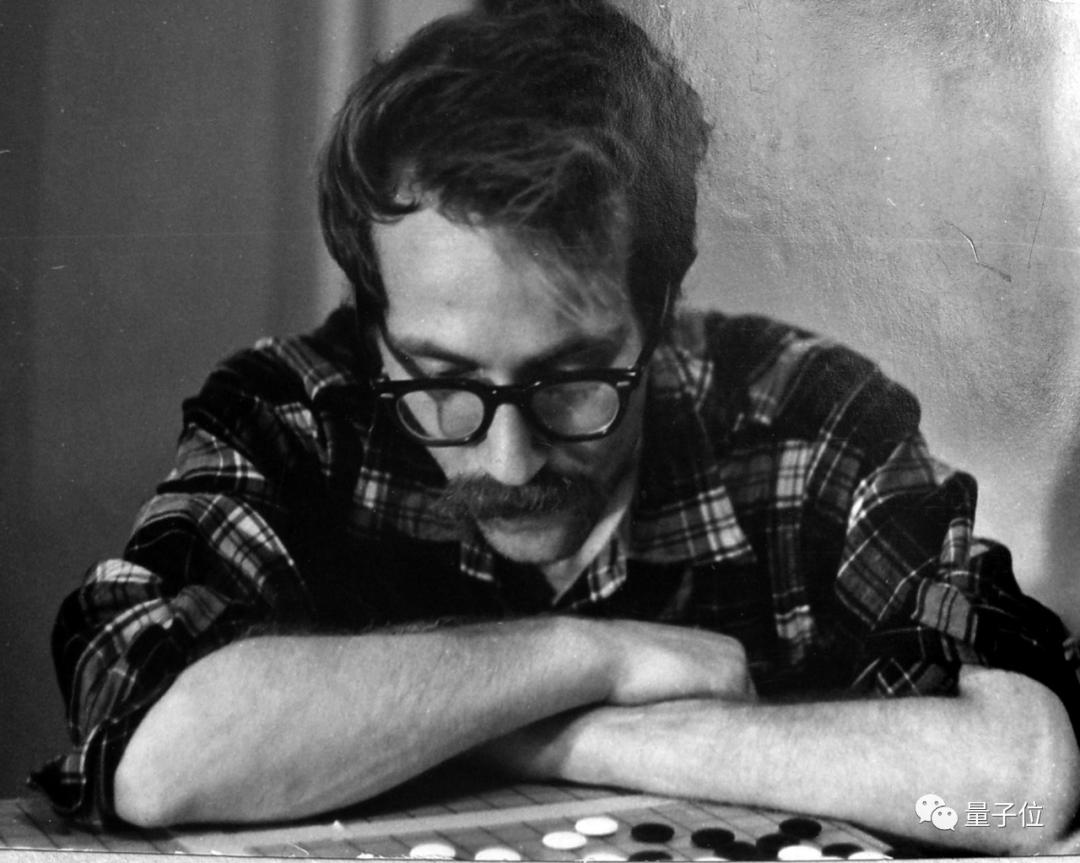
\includegraphics[scale=0.2]{weizner}
  \caption{젊은 날의 와이즈너}
\end{figure}

\noindent
와이즈너는 이 이야기를 \snm{켤레 코딩}{\tiny Conjugate Coding}이라는 논문으로
정리해 유명한 정보이론 저널에 보냈다. 저널은 \snm{켤레 코딩}을 거절했다.
정보학자들이 물리학자의 어투를 낯설게 여긴 탓이다. 와이즈너는 머지 않아 학계를
떠났다. 그리고 베유{\tiny Simon Weil}처럼 육체 노동의 가치를 찬미하며 건설
노동자로 여생을 보냈다.

한편 베넷은 와이즈의 이야기를 잊지 않았다. 계속 이야기하고 다녔다. 그러다 
몬트리올 출신 암호학자 브라사르{\tiny Gilles Brassard}가 재밌게 들었다. 
베넷과 브라사르는 상이한 배경에도 불구하고 즐겁게 이야기를 나눴다. 
그리고 1982년 \snm{양자 암호학, 혹은 복제 불가능한 지하철 승차권}{\tiny
Quantum Cryptography, or Unforgeable Subway Tokens}이라는 논문을 내놓았다. 
이 논문이 이룬 업적 가운데 하나는 바로 1983년 ACM 뉴스레터로 하여금 \snm{켤레
코딩}을 싣도록 유도한 것이다. 

\snm{켤레 코딩}에 따르면 해커는 어느 미지의 큐비트와 동일한 양자 상태의
두 번째 큐비트를 복제할 수 없다. 또 위조할 수 없는 화폐가 존재할 수 있다.
복사불능정리 덕이다. 다시 말해 양자정보라는 분야는 커녕 `큐비트'라는 말조차
없던 시절 복사불능정리를 당연하게 받아들이고 양자화폐와 양자암호라는 응용
분야를 개척한 10쪽 짜리 논문이 바로 \snm{켤레 코딩}이다.

양자은행이 존재하여 양자지폐를 찍어낸다고 하자. 각 양자지폐는 고전적인 
일련번호 $s\in\{0,1\}^n$와 양자상태 $\ket{\psi_{f(s)}}$를 지닌다. 이때
$\ket{\psi_{f(s)}}$상의 큐비트들은 얽혀있지 않고 아래 네 상태 가운데
하나를 지닌다. 얽혀있지 않다는 조건을 부여하는 이유는 $\ket{\psi_{00}}$을 
알더라도 얽힘에 의해 나머지 $\ket{\psi_{ij}}$는 알 수 없도록 하기 위해서다.
\[
  \ket{\psi_{00}}=\ket0,\ket{\psi_{01}}=\ket1,\ket{\psi_{10}}=\ket+,
  \ket{\psi_{11}}=\ket-
\]
양자은행은 일련번호 $s$와 양자지폐가 지녀야 하는 양자상태상의 각 큐비트들의
기저를 부호화한 문자열 $f(s)$를 저장하고 있다. 복사불능정리로 인해
양자상태 $\ket{\psi_{f(s)}}$를 복사하여 위조하는 작업은 당연히 불가능하다. 
문제는 양자지폐를 어떻게 검증{\tiny verify}하냐는 것이다.

우선 양자지폐를 양자은행에 갖다준다. 양자은행은 검증하려는 양자지폐의 일련번호
$s$에 따른 $f(s)$를 준비한다. 그리고 검증하려는 양자지폐의 양자상태 속 각
큐비트를 차례로 $f(s)$로 관측한다. 양자지폐가 진짜라면 관측이 매끄럽게 진행될
것이고 양자지폐가 가짜라면 관측 도중 특정 큐비트 $\ket{\phi_x}$에 대해 이상한
관측 결과가 나올 것이다. 물론 위폐범이 그냥 기저를 때려 맞춰서 양자지폐를
위조할 수 있겠지만 이게 먹힐 확률은 $n$번 찍는다고 했을 때 
$\left(\frac{1}{2}\right)^n$이다. 사실상 불가능하다.

그러나 바로 이게 문제다. 양자지폐를 사용하려고 할 때마다 양자은행의 검증이
필요하다면 애초에 양자지폐를 사용할 이유가 없다. 거래 과정에서 은행의 개입을
요구하지 않는다는 현금의 최대 장점이 쏙 빠진 셈이다. 

그리하여 \emph{공개키\tiny public-key}를 도입할 수도 있겠다. 모든 사람이
\emph{공개키}로 양자지폐를 검증할 수 있도록 허락하고 \emph{개인키}를 지닌
양자은행만 양자지폐를 생산할 수 있도록 제한하는 방법이다. 
하지만 위조범이 엄청난 계산 능력을 지녀서 그냥 있을 수 있는 양자 상태를
다 때려박으면 공개키 검증 절차를 통과하는 양자 상태를 찾아낼 수도 있다. 

이에 1984년 베넷과 브라사드는 \snm{켤레 코딩}의 유산인 \textbf{양자 키
분배\tiny quantum key distribution}를 고안한다. 베넷과 브라사드가 1984년
발표한 방법이라 \textbf{BB84 프로토콜}이라고 부른다. BB84는 아래와 같은 
프로토콜이다.
\begin{mdframed}
\begin{enumerate}[label=(\Alph*)]
  \item 앨리스가 문자열의 쌍 $x,y\in\{0,1\}^n$를 무작위로 고른다. 가령 $x$가
    $010\cdots010$이고 $y$가 $111\cdots110$일 수 있다.
  \item 앨리스는 $n$개의 큐비트로 구성된 양자상태 $\ket{\psi}$를 다음 절차로
    생성한다. 
    \begin{enumerate}[label=(\roman*)]
      \item 큐비트를 부호화할 기저는 $y$로 결정한다. 
    $0$에는 $\{\ket0,\ket1\}$, $1$에는 $\{\ket+,\ket-\}$로 결정한다.
    $y=111\cdots110$에 대해 첫 세 큐비트는 $\{\ket+,
    \ket-\}$를 기저로 부호화하고 마지막 큐비트는 $\{\ket0,\ket1\}$를 기저로 
    부호화하는 식이다. 
      \item 그리고 $x$로 주어진 기저에 대해 원소를 결정한다.
    $0$에는 기저에 따라 $\ket0$ 혹은 $\ket+$, $1$에는 기저에 따라 $\ket1$ 혹은
    $\ket-$로 결정한다. 가령 $x=010\cdots010$에 대해 첫 큐비트는 $\ket+$로,
    두 번째 큐비트는 $\ket-$로, 마지막 큐비트는 $\ket0$으로 결정하는 식이다.
  \end{enumerate}
  \item 이제 앨리스는 밥에게 양자상태 $\ket{\psi}$를 송신한다. 
  \item 밥은 $\{0,1\}^n$에서 무작위로 문자열 $y'$을 고른다. 그리고 
    \begin{enumerate}[label=(\roman*)] 
      \item 수신한 $\ket{\psi}$의 각 큐비트를 측정할 기저를
  $y'$로 결정한다. $0$에는 $\{\ket0,\ket1\}$로 측정하고, $1$에는 $\ket+,\ket-\}$로
  측정하는 것이다. 
    \item 측정 결과가 나타나면 $\ket0$이나 $\ket+$에
    대해 $0$을, $\ket1$이나 $\ket-$에 대해 $1$을 문자열 $x'$로 기록한다.
  \end{enumerate}
  \item 이제 앨리스와 밥은 $y$와 $y'$를 공유한다. 그리고 둘은 같은 기저를
    고르지 않은 $y$와 $y'$의 성분에 대한 $x$와 $x'$의 성분을 전부 버린다.
    대략 절반의 비트이며, 그리하여  $x$와 $x'$로 남는 것이 공유 비밀키다.
  \item 공유 비밀키가 존재하며 양자역학이 보안을 보장한다. 그리하여 
    공유 비밀키를 일회성 패드 같은 고전적인 암호 체계에 사용하면 된다.
\end{enumerate}
\end{mdframed}
염탐자 이브가 있다고 하자. 일단 이브는 복사불능정리에 의해 $\ket{\psi}$를
갈취할 수 없다. 그러니 이브는 $\ket{\psi}$를 면밀히 관측할
것이다. 그러나 이브는 각 $\ket{\psi_i}$의 기저를 모른다. 한 번
정도는 때려 맞힐 수 있겠지만 한 번이라도 틀리면 $\ket{\psi}$ \emph{자체}가
변모한다. 그리하여 염탐자가 존재하거나 존재하지 않는다는 사실을 보장할
수 있다. $y$와 $\ket{\psi}$의 분포가 판이하면 염탐자가 존재했다는 뜻이기 때문이다.

그리고 $y$는 고전적인 문자열이니까 이브가 갈취하거나 면밀히 관찰할 수도 있다.
상관 없다. $y$와 $y'$의 교환은 $\ket{\psi}$를 보낸 다음에 이루어지기
때문이다. 열심히 갈취한 $y$는 아무 짝에도 쓸모가 없다. BB84의 골자는
누가 기밀을 엿듣든 말든 양자역학에 의해 상관 없다는 것이다.
\chapter{얽힘}
정보이론에 따르면 $n$비트를 보낼 때 $n$비트 이상의 정보를 송신할 수는
없다. 한편 앨리스와 밥은 큐비트 하나로 고전 비트 두 개를 보낼 수 있다.
물론 우선 앨리스와 밥이 얽힘을 공유해야 한다. 이런 얽힘을 미리
공유하지 않았다면 앨리스는 큐비트 하나당 하나의 비트만 보낼 수 있다. 이를
\textbf{홀레보{\tiny Holevo}의 정리}라고 부른다. 만약 앨리스가 $\ket{\psi}=
\alpha\ket0+\beta\ket1$을 밥에게 보낸다면 밥은 $\ket{\psi}$를 오직 한 번만
측정할 수 있고 $\ket{\psi}$상의 나머지 정보는 유실된다.

앨리스와 밥이 벨 쌍 $\ket=\frac{\ket{00}+\ket{11}}{\sqrt2}$를 미리 공유한다고
하자.
\end{document}
